\section{Initial Investigations}

The contents of this section explain the approach, methodology, and results of the initial investigations using machine learning to infer the signal-to-interference of a single radio link using situational awareness information from a camera system as published in~\cite{CandellISIE2019.Conf} with data made available~\cite{https://doi.org/10.18434/m32077}.

\subsection{Data Analysis}\label{ftml-conf:sec:dataanalysis}

%	\begin{figure}[tbp]
%	    \centering
%	    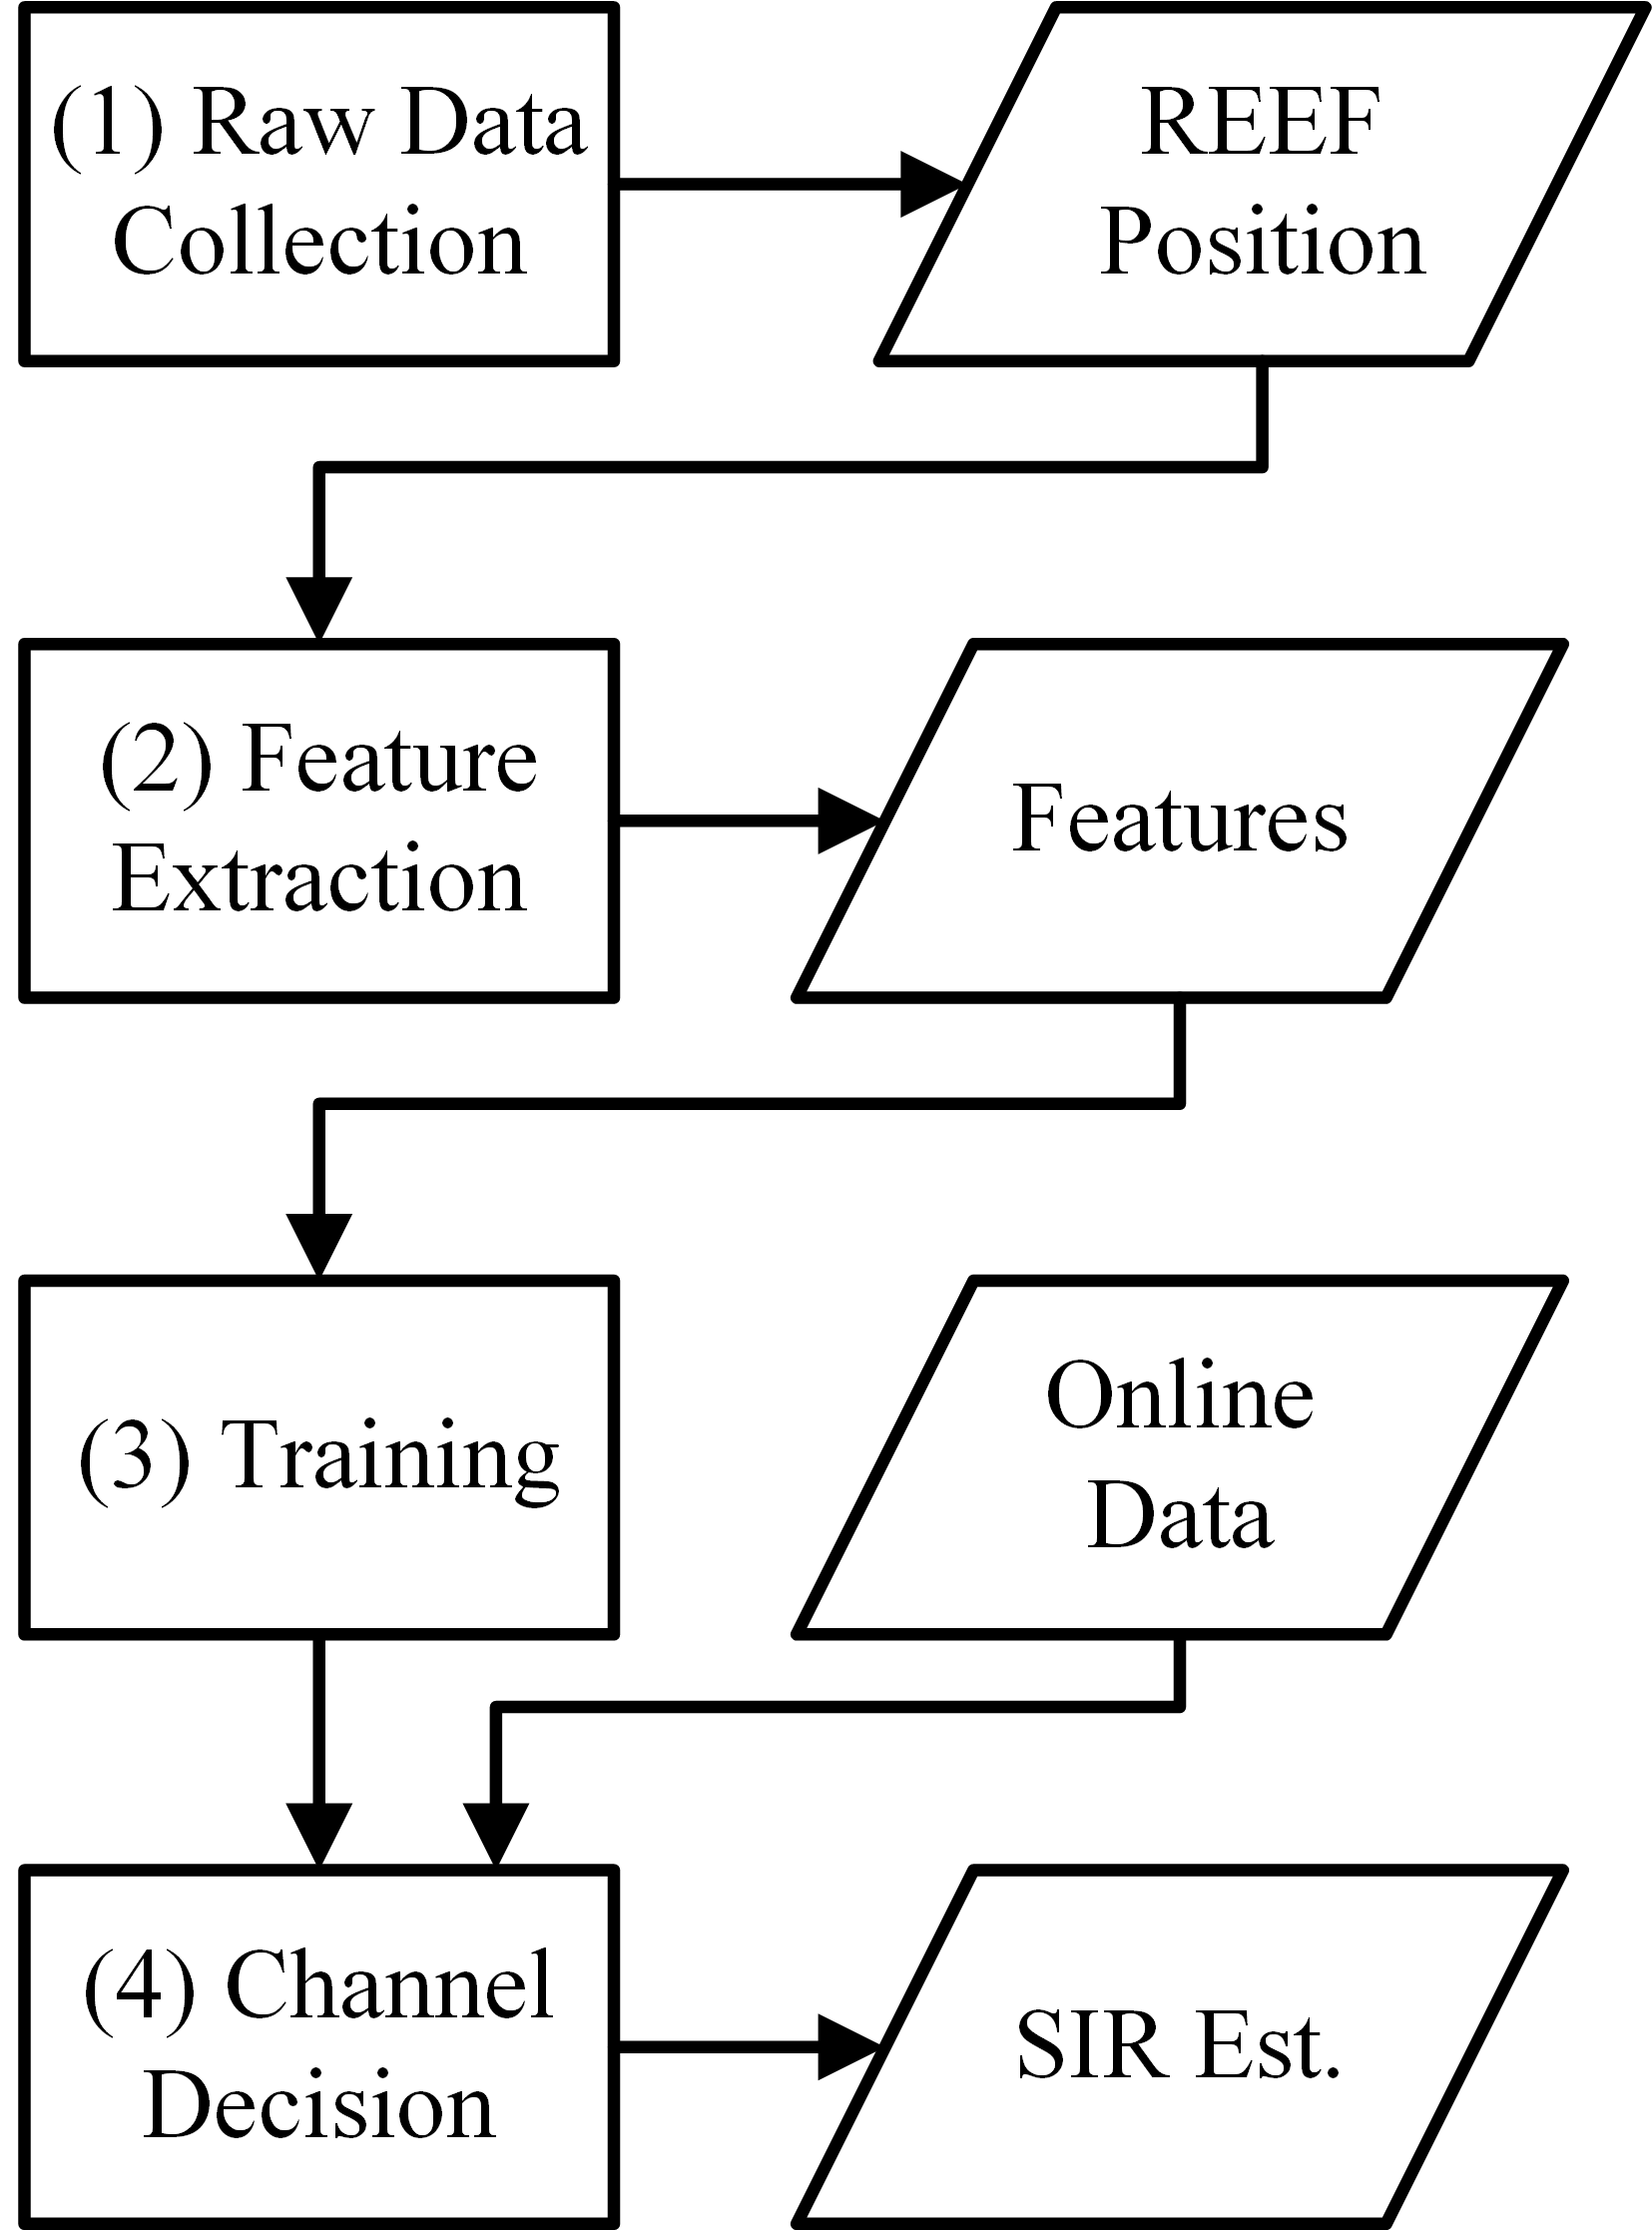
\includegraphics[width=0.65\columnwidth]{diagrams/DataFlow-verticle}
%	    \caption{Data analytics includes raw data capture from a vision system, feature extraction, training, and  operation.}
%	    \label{ftml-conf:fig:dataflow}
%	\end{figure}

The data analysis process for the experiment
%was conducted according to the diagram in Fig.~\ref{ftml-conf:fig:dataflow} and 
is divided into four parts: raw data collection, data cleaning and feature extraction, training, and the operation of the SIR estimation.  The raw data was produced as an output of the VTS as a time series of z-axis position.  Feature extraction was conducted in MATLAB by following the time series and extracting or calculating features for each iteration.  Once features were extracted, a statistical analysis of the features was conducted to determine the variability of the features as a function of SIR.  Statistical analyses included visual inspection of histograms of each factor and an inspection of the correlation coefficients over the range  of SIRs.  A discussion of the statistical results is provided in~\ref{ftml-conf:sec:results:stats} which demonstrates suitability of the use of position measurements for machine learning. Training of a machine learning algorithm followed. The machine learning algorithm was programmed in Python using the Sci-kit Learn library~\cite{SCIKITLEARN}.

\subsection{Feature Extraction}\label{ftml-conf:sec:data:feats}

%\begin{figure}[tbp]
% \centering
%	\subfloat[sample time series of probe position\label{ftml-conf:fig:timeseries-zplot}]{%
%		\includegraphics[width=0.8\columnwidth]{plots/timeseries-zplot}}
%	\hfill
%	\subfloat[feature extraction model\label{ftml-conf:fig:timeseriesfeatures}]{%
%		\includegraphics[width=0.9\columnwidth]{diagrams/timeseries.png}}
%	\caption{A time-series sample~\subref{ftml-conf:fig:timeseries-zplot} of a single iteration of the measured z-axis probe position and~\subref{ftml-conf:fig:timeseriesfeatures} the corresponding model for feature extraction.}
%	\label{ftml-conf:fig:timeseries-and-model}      
%\end{figure}	

\begin{figure}[!ht]
	
	\centering
	
	\begin{subfigure}{.95\textwidth}
		\centering
		% include first image
		\includegraphics[]{./chapter-ftml/plots/timeseries-zplot}  
		\caption{sample time series of probe position in mm}
		\label{ftml-conf:fig:timeseries-zplot}
	\end{subfigure}
	
	\begin{subfigure}{.95\textwidth}
		\centering
		% include second image
		\includegraphics[]{./chapter-ftml/diagrams/timeseries.png}  
		\caption{feature extraction model}
		\label{ftml-conf:fig:timeseriesfeatures}
	\end{subfigure}
	
	\caption{A time-series sample~\protect\subref{ftml-conf:fig:timeseries-zplot} of a single iteration of the measured z-axis probe position and~\protect\subref{ftml-conf:fig:timeseriesfeatures} the corresponding model for feature extraction.}
	\label{ftml-conf:fig:timeseries-and-model}
	
\end{figure}

Feature extraction begins with a time series of position of the probe through successive iterations of the plunger applying force to the spring and then returning to its home position.  A sample time series of the z-axis position of the probe is as shown in~Fig.~\ref{ftml-conf:fig:timeseries-zplot}.  Rather than using the time series directly, a more convenient and practical solution is to extract features that represent aspects that may be useful for analysis and machine learning algorithms.  This reduces the number of learning dimensions and usually improves computation efficiency.  The selected features are illustrated in~Fig.~\ref{ftml-conf:fig:timeseriesfeatures}.   Shown in the model, the probe begins at its home position, \textbf{a}.  It will not begin its downward motion until it receives sufficient FTS readings.  Marker \textbf{b} indicates the beginning of the probes descent.  Marker \textbf{c} represents that point in which the probe descends below a predetermined threshold, and marker \textbf{d} represents the position in which the probe begins its return ascent to the home position.  Finally the probe returns to the home position as indicated by marker \textbf{e}.  Therefore, the extracted features of each successive iteration is defined as follows:

\begin{description}
    \item[Feature $Z_d$] The length of the probe's descent measured in millimeters,
    \item[Feature $\Delta{t}_{ab}$] The duration in seconds the the robot waits before moving the probe along its descent,
    \item[Feature $\Delta{t}_{bc}$] The duration in seconds of the time that the robot takes to move the probe beyond the threshold, $Z_{th}$, of -77 mm,
    \item[Feature $\Delta{t}_{cd}$] The duration in which the probe dwells below $Z_{th}$ and the speed of the probe remains under 0.15 mm/sec,
    \item[Feature $\Delta{t}_{ae}$] The duration of the full iteration as measured from the home position, \textbf{a}, to the next home position, \textbf{e}.
\end{description}


\subsubsection{Statistical Analysis}\label{ftml-conf:sec:data:stats}
Each factor was visually examined to assess its variability as a function of the SIR.  In order to predict the SIR given a set of measurements of the dynamics of the physical system, sufficient variability is needed.  This assessment was performed visually using histograms as a basis for comparison.  The factors $Z_{d}$ and $\Delta{t}_{bc}$ were used for examination of the data using histograms.  

In addition, it would be helpful to show that the factors are uncorrelated as a function of SIR demonstrating a further level of confidence that each factor will be useful to a machine learning algorithm.  This assessment was accomplished by computing the correlation coefficient matrix of the extracted factors as defined by the Pearson product-moment method~\cite{Yeager}.  The correlation coefficient matrix is a covariance matrix that is normalized by the product of the standard deviations of two factors being compared according to $\rho_{X,Y} = cov(X,Y)/(\sigma_{X}\sigma_{Y})$.	Since each factor correlates exactly with itself, a correlation matrix should have values of 1 along the diagonal.  Other elements of the matrix will take on values between -1 and 1.  A visual inspection of the coefficient matrices will show how strongly selected factors vary together.  Correlation can be viewed as a function of SIR to verify that factors are independently applicable to a learning algorithm.  The objective of factor selection is, therefore, to choose factors that are highly uncorrelated and yet still vary appreciably\cite{LeeRodgers1988}.

\subsubsection{Machine Learning}\label{ftml-conf:sec:data:ML}
In order to learn the SIR level from observing the various features, the random forest model is leveraged~\cite{Breiman2001}. Random forest is an ensemble of decision trees with random feature selection which can be used for classification or regression based on the predicted output space. Deploying random forest in machine learning has been successful in various applications such as described in \cite{Zhen2015},~\cite{Shotton2011}, and~\cite{Zhen2014}. Its main advantages are that it is stable, fast to compute, and insusceptible to over-fitting.

In this work, the random forest model is deployed for SIR regression using the five features defined in \ref{ftml-conf:sec:data:feats}. These features are evaluated for each iteration of the probe movement. A data segment is defined which is composed of a number of successive iterations.  The segment size is denoted by $M$. As a result, the random forest regression model is used to get an input vector of size $5M$ and regression output of the corresponding SIR value. The random forest is selected because it is computationally efficient with high-dimensional data and it is robust for outliers and data non-linearity. 

The random forest regression model is first trained by taking a fixed number of segments for each SIR labelled data. The size of the training set for each SIR level is denoted by $T$. The rest of the measurements are used for testing. In general, the proposed machine learning approach will deploy a sliding window approach of size $M$ to collect the features of the force-seeking use case to estimate the current level of SIR at various nodes of the wireless network. 

\subsection{Results} \label{ftml-conf:sec:results}  

The results in this section are  presented from an experimental run in which the jammer \textbf{J} interferes with the router, \textbf{R}, while communication is conducted using a mixed mode of IEEE 802.11 b and g~\cite{IEEE802.11ac}.  Analyses using histograms and covariance are presented in Section~\ref{ftml-conf:sec:results:stats} followed by results of the machine learning application in Section~\ref{ftml-conf:sec:results-ML}.

\subsubsection{Statistical Analysis}\label{ftml-conf:sec:results:stats}
\paragraph{Analysis of Factors Using Histograms}

%\begin{figure}[tbp]
% \centering
%	\subfloat[z-axis position\label{ftml-conf:fig:results-zpos-hist}]{%
%		\includegraphics[width=0.8\columnwidth]{plots/ZPosHists}}
%	\hfill
%	\subfloat[Plunge delay $\Delta{t}_{bc}$\label{ftml-conf:fig:results-dtbc-hist}]{%
%		\includegraphics[width=0.8\columnwidth]{plots/DeltaTbc.png}}
%	\caption{Variations in probability distributions of the z-axis position \subref{ftml-conf:fig:results-zpos-hist} and the plunge delay \subref{ftml-conf:fig:results-dtbc-hist} indicate that machine learning may be effective in inferring information about the underlying communication channel. In the figure, the baseline case of infinite SIR is depicted as a histogram with white bars, and the experimental case is depicted as a histogram with red bars.}
%	\label{ftml-conf:fig:results-hists}      
%\end{figure}

\begin{figure}[!ht]
	\centering
	\begin{subfigure}{.75\textwidth}
		\centering
		% include first image
		\includegraphics[width=.8\linewidth]{./chapter-ftml/plots/ZPosHists}  
		\caption{z-axis positione}
		\label{ftml-conf:fig:results-zpos-hist}
	\end{subfigure}
	\begin{subfigure}{.75\textwidth}
		\centering
		% include second image
		\includegraphics[width=.8\linewidth]{./chapter-ftml/plots/DeltaTbc.png}  
		\caption{Plunge delay}
		\label{ftml-conf:fig:results-dtbc-hist}
	\end{subfigure}
	\caption{Variations in probability distributions of the z-axis position~\protect\subref{ftml-conf:fig:results-zpos-hist} and the plunge delay~\protect\subref{ftml-conf:fig:results-dtbc-hist} indicate that machine learning may be effective in inferring information about the underlying communication channel. In the figure, the baseline case of infinite SIR is depicted as a histogram with white bars, and the experimental case is depicted as a histogram with red bars.}
	\label{ftml-conf:fig:results-hists}
\end{figure}



The results of the histogram analyses for the z-axis position of the probe and the probe descent delay are shown in Fig.~\ref{ftml-conf:fig:results-zpos-hist} and Fig.~\ref{ftml-conf:fig:results-dtbc-hist}, respectively.  The expectation of the histogram analysis was that $Z_d$ and the $\Delta{T}_{bc}$ would exhibit appreciable variation that may be observed through a visual inspection.  This was indeed the case.  Referring to Fig.~\ref{ftml-conf:fig:results-zpos-hist}, a visual inspection reveals that the minimum z-axis position for each iteration skews to lower positions for lower SIR values and higher positions for higher SIR values.  This implies that the controller algorithm responds faster to force sensor readings at higher SIR values than lower values.  Similarly, by observing the plunge delay, $\Delta{t}_{bc}$, the controller takes more time to respond at lower SIR values than at higher values.  This behavior is exemplified by the probability skew shown in the histograms. 

\paragraph{Factor Correlation Coefficient Analysis}

\begin{table}[!ht]

   	\centering
   	\caption{Correlation Coefficients for $-9\ dB$ SIR}
   	\label{ftml-conf:tab:m9corrcoeff}
   	\begin{tabular}{|l|c|c|c|c|c|}
\hline
&\textbf{$\Delta{t}_{ab}$}&\textbf{$\Delta{t}_{bc}$}&\textbf{$Z_d$}&\textbf{$\Delta{t}_{cd}$}&\textbf{$\Delta{t}_{ae}$}\\\hline
\textbf{$\Delta{t}_{ab}$}&1&0.04&0.04&0&0.56\\\hline
\textbf{$\Delta{t}_{bc}$}&0.04&1&-0.96&-0.08&0.18\\\hline
\textbf{$Z_d$}&0.04&-0.96&1&0.03&-0.01\\\hline
\textbf{$\Delta{t}_{cd}$}&0&-0.08&0.03&1&0\\\hline
\textbf{$\Delta{t}_{ae}$}&0.56&0.18&-0.01&0&1\\\hline
\end{tabular}

   	\vspace{5mm}

   	\centering
   	\caption{Correlation Coefficients for $-8\ dB$ SIR}
   	\label{ftml-conf:tab:m8corrcoeff}
   	\begin{tabular}{|l|c|c|c|c|c|}
\hline
&\textbf{$\Delta{t}_{ab}$}&\textbf{$\Delta{t}_{bc}$}&\textbf{$Z_d$}&\textbf{$\Delta{t}_{cd}$}&\textbf{$\Delta{t}_{ae}$}\\\hline
\textbf{$\Delta{t}_{ab}$}&1&0.01&-0.05&-0.06&0.58\\\hline
\textbf{$\Delta{t}_{bc}$}&0.01&1&-0.99&-0.13&0.1\\\hline
\textbf{$Z_d$}&-0.05&-0.99&1&0.07&-0.1\\\hline
\textbf{$\Delta{t}_{cd}$}&-0.06&-0.13&0.07&1&-0.03\\\hline
\textbf{$\Delta{t}_{ae}$}&0.58&0.1&-0.1&-0.03&1\\\hline
\end{tabular}

   	\vspace{5mm}

   	\centering
   	\caption{Correlation Coefficients for $-7\ dB$ SIR}
   	\label{ftml-conf:tab:m7corrcoeff}
   	\begin{tabular}{|l|c|c|c|c|c|}
\hline
&\textbf{$\Delta{t}_{ab}$}&\textbf{$\Delta{t}_{bc}$}&\textbf{$Z_d$}&\textbf{$\Delta{t}_{cd}$}&\textbf{$\Delta{t}_{ae}$}\\\hline
\textbf{$\Delta{t}_{ab}$}&1&-0.05&-0.04&0.09&0.01\\\hline
\textbf{$\Delta{t}_{bc}$}&-0.05&1&-0.93&-0.17&0.05\\\hline
\textbf{$Z_d$}&-0.04&-0.93&1&0.08&-0.05\\\hline
\textbf{$\Delta{t}_{cd}$}&0.09&-0.17&0.08&1&-0.02\\\hline
\textbf{$\Delta{t}_{ae}$}&0.01&0.05&-0.05&-0.02&1\\\hline
\end{tabular}


\end{table}

Correlation coefficients were calculated for each of the five factors defined in Section~\ref{ftml-conf:sec:data:feats} and correlation coefficients matrices were produced for each of the SIR values used.  The correlation coefficient matrices for SIR values of -9, -8, and -7 are shown in Tables~\ref{ftml-conf:tab:m9corrcoeff}-\ref{ftml-conf:tab:m7corrcoeff}, respectively. Inspection of the correlation coefficient tables indicate that the factors are mostly uncorrelated across SIR values except for the clear correlation between plunge delay and plunge depth. Low correlation values demonstrate a necessary but not sufficient condition for the independent applicability factors to machine learning.  If desired, either $\Delta{t}_{bc}$ or $Z_d$ could be omitted as they are strongly correlated and therefore provide redundant information.

\subsubsection{Machine Learning Results}\label{ftml-conf:sec:results-ML}
The proposed machine learning approach is deployed for three values of the SIR, -9, -8, and -7 dB. First the output of the random forest regression model for two values of the segment size $M$ is shown. The training set size $T=200$ is set for each SIR value. The random forest model is used with a number of estimators of 500 and a tree depth of 5. In Fig.~\ref{ftml-conf:fig:results-BP}, the box plots of the predicted SIRs are presented against the correct value of the corresponding SIR for $M=100$ and $M=1$.  Generally, increasing the value of $M$ increases the acquisition time for the input data for the random forest model while enhancing the performance of the algorithm. By setting $M=1$, it is evident the predicted values of SIR are widely spread around the median and a large number of outliers exists. However, increasing $M$ reduces variations in the predicted SIRs and a smaller number of outliers.


%\begin{figure}[tbp]
%	\subfloat[$M=100$\label{ftml-conf:fig:results-BP-1}]{%
%		\includegraphics[width=\columnwidth]{plots/BP_1}}
%	\hfill
%	\subfloat[$M=1$\label{ftml-conf:fig:results-BP-2}]{%
%		\includegraphics[width=\columnwidth]{plots/BP_2}}
%	\caption{Predicted SIR versus actual SIR for the cases of~\subref{ftml-conf:fig:results-BP-1} $M=100$ and~\subref{ftml-conf:fig:results-BP-2} $M=1$. The box plots show the median value while the bottom and top edges of the box indicate the 25th and 75th percentiles.  Statistical outliers are shown as red $+$ signs.}
%	\label{ftml-conf:fig:results-BP}      
%\end{figure}

\begin{figure}[!ht]
	\begin{subfigure}{.5\textwidth}
		\centering
		% include first image
		\includegraphics[width=.8\linewidth]{./chapter-ftml/plots/BP_1}  
		\caption{[$M=100$}
		\label{ftml-conf:fig:results-BP-1}
	\end{subfigure}
	\begin{subfigure}{.5\textwidth}
		\centering
		% include second image
		\includegraphics[width=.8\linewidth]{./chapter-ftml/plots/BP_2}  
		\caption{[$M=1$}
		\label{ftml-conf:fig:results-BP-2}
	\end{subfigure}
	\caption{Predicted SIR versus actual SIR for the cases of~\protect\subref{ftml-conf:fig:results-BP-1} $M=100$ and~\protect\subref{ftml-conf:fig:results-BP-2} $M=1$. The box plots show the median value while the bottom and top edges of the box indicate the 25th and 75th percentiles.  Statistical outliers are shown as red $+$ signs.}
	\label{ftml-conf:fig:results-BP}
\end{figure}

In Fig.~\ref{ftml-conf:fig:prediction-error}, the two criteria for measuring the performance of the proposed SIR estimation algorithm is presented. The performance against the segment size $M$ is shown. The first criterion is the mean squared error where the mean of the squared error between the estimated SIR and the actual SIR values is calculated. The second criterion is the variance score which is a statistical measure of how close the data are to the fitted regression line. The r-squared variance score is used which is defined as the ratio between the total variance explained by model and total variance of the data \cite{r-squared}. In this figure the improvement in the performance against the segment size is demonstrated. 

\begin{figure}[tbp]
 \centering
 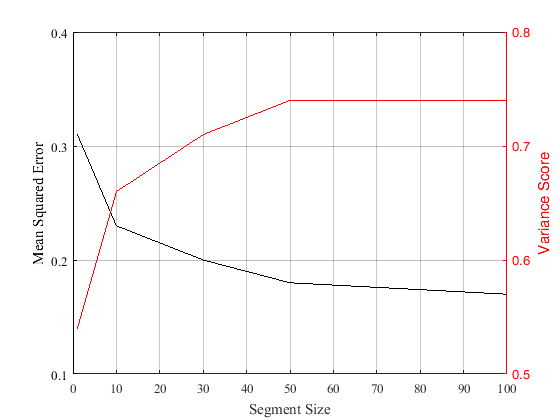
\includegraphics[width=0.75\columnwidth]{./chapter-ftml/plots/prediction-error}
 \caption{The performance of the random forest regression model against $M$.}
 \label{ftml-conf:fig:prediction-error}
\end{figure}

\subsection{Conclusion}\label{ftml-conf:sec:conclusion}

This investigation presented a practical use case of a wireless force-torque feedback control system that could be deployed in a manufacturing assembly system such as a pick-and-place or assembly operation.  A 6-DOF force sensor was connected to a robot controller tasked with moving a probe along a linear path until an opposing force exceeding 5 N was detected.  It is demonstrated that the reliability of the wireless communication system directly impacts the repeatability performance of the physical system. It is also demonstrated that the quality of the underlying wireless channel may be inferred by observing the position of the probe along a single spatial dimension and applying machine learning to predict the signal-to-interference ratio. The findings provide motivation for applying machine learning to larger more complex systems with high degrees of freedom. Future work will extend to the inclusion of more descriptive factors, the addition of network information such as the wireless protocol mode, and the addition of a larger number of variables tracked by many remote observers. Experimentation with neural networks and deep learning to improve prediction accuracy and better generalization will be of great values to wireless operations in factories.  Finally, the applications of online machine learning techniques to this and other use cases could provide significant benefits to the manufacturing community.



